\documentclass[12pt]{article}
\usepackage{latexsym}
\usepackage{epsfig}
\usepackage{tikz}
\usetikzlibrary{arrows}

\setlength{\topmargin}{0in}
\setlength{\leftmargin}{0in}
\setlength{\textwidth}{6in}
\setlength{\textheight}{9.5in}
\setlength{\parindent}{0.2in}
\setlength{\parskip}{.08in}
\voffset = -.45in
\hoffset = -.5in

\begin{document}
\newcommand{\lsp}[1]{\large\renewcommand{\baselinestretch}{#1}\normalsize}

\lsp{1}
\pagestyle{plain}
\begin{center}
{\bf
Maze Worksheet
}
\end{center}

\begin{flushleft}
   Consider the following maze:
\end{flushleft}

\begin{center}
   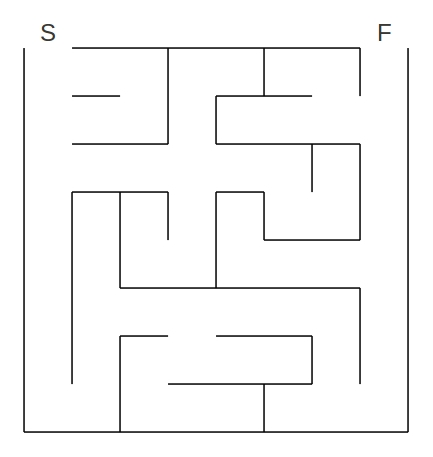
\includegraphics[width=3in]{./maze.jpg}
\end{center}
\begin{flushleft}
   Show how to model the maze as a graph.

   Each intersection of the maze could be represented as a vertex and the
   routes between them as edges. This would allow you to use the BFS and DFS
   algorithms to find the solution.
\end{flushleft}
\begin{center}
   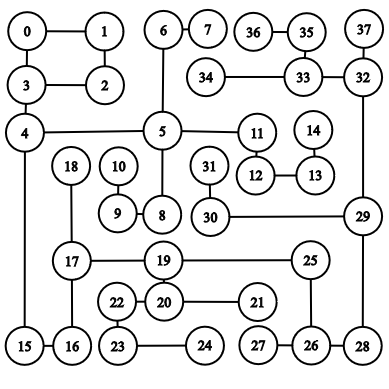
\includegraphics[width=3in]{./graph.png}
\end{center}

\pagebreak
\begin{flushleft}
   Perform a breadth-first search on the maze to show how this algorithm can be used to find the shortest path from start to finish.
\end{flushleft}
\begin{center}
   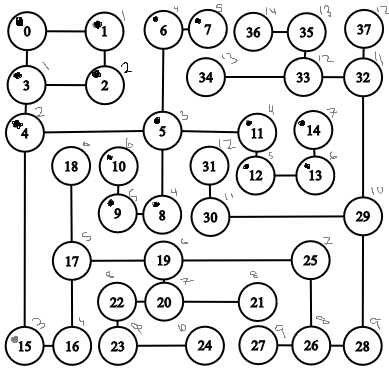
\includegraphics[width=3in]{./graph-annotated.png}
\end{center}
The shortest path takes 12 hops and is as follows:

$0 \to 3 \to 4 \to 15 \to 16 \to 17 \to 19 \to 25 \to 26 \to 28 \to 29 \to 32 \to 37$
\end{document} 
